\section{Einleitung}
 In diesem Kapitel wird die Auftragsgeberfirma Colomba Link vorgestellt. Es wird die Ausgangs
lage beschrieben und das zu lösende Problem wird eingeführt. Es werden grundlegende Begriffe
 definiert, die in dieser Thesis von Bedeutung sind.

\subsection{Colomba Link}

Die Colomba Link GmbH entwickelt mit Monidas eine IoT-Plattform zur Vernetzung, Verwaltung und Auswertung industrieller Anlagendaten. Sie richtet sich an IoT-Spezialisten sowie Endnutzer und bietet Funktionen von der Einrichtung der Sensoren bis zur automatisierten Überwachung und Alarmierung. Derzeit konfigurieren technische Mitarbeitende die Sensoren kundenspezifisch über eine Weboberfläche (Monidas-Plattform). Komponenten wie Sensoren, Regeln und Benachrichtigungen müssen dabei einzeln erstellt und anschliessend manuell über mehrere Eingabemasken miteinander verknüpft werden. Mit zunehmender Anzahl von Sensoren steigt dadurch der Aufwand für das technische Personal. Aufgrund begrenzter Entwicklungsressourcen verfolgt das Startup das Ziel einer generischen Implementierung, welche Anpassungen und Erweiterungen des Datenmodells sowie den Verwaltungsprozess erleichtert und langfristig zu höherer Kundenzufriedenheit beiträgt. 

\subsection{Konfigurationsprozess}
Zum Verständnis der in dieser Arbeit beschriebenen Lösung ist es erforderlich, den Aufbau und die Konfiguration der Sensoren in der Monidas-Plattform grundlegend zu kennen. Der folgende Abschnitt erläutert den aktuellen Ablauf der Sensorkonfiguration und stellt relevante Begriffe vor. Dabei beschränkt sich die Darstellung auf jene Aspekte, die für die Problemstellung und die entwickelte Lösung von Bedeutung sind.

Die Konfiguration eines Sensors auf der Monidas-Plattform erfolgt über Eingabemasken. Dabei handelt es sich um Benutzeroberflächen, auf denen Informationen eingegeben und Optionen ausgewählt werden können. Erst wenn alle erforderlichen Konfigurationselemente erstellt wurden, können sie im Monitor zusammengeführt werden. Dieser verknüpft sämtliche Elemente miteinander und ermöglicht dadurch die Überwachung des Sensors.

Im Folgenden werden die einzelnen Konfigurationselemente näher beschrieben:

Actions definieren, wann und unter welchen Bedingungen eine Benachrichtigung versendet wird. Eine Benachrichtigung ist eine Mitteilung, die an vordefinierte Empfängergruppen gesendet wird. Dabei kann festgelegt werden, dass eine Benachrichtigung bei bestimmten Sensorzuständen (Idle, Alert oder Alarm) ausgelöst wird. Zusätzlich wird konfiguriert, ob die Benachrichtigung bei jedem Auftreten des Zustands oder nur einmalig versendet werden soll. Eine Benachrichtigung setzt sich aus den Konfigurationselementen Gruppe und Template zusammen.

Groups sind Vorlagen, in denen definiert ist, an welche Empfänger eine Benachrichtigung gesendet wird. Die entsprechenden E-Mail-Adressen werden innerhalb der Gruppe hinterlegt. Aktuell unterstützt die Plattform ausschließlich den Kommunikationskanal E-Mail.

Templates sind Vorlagen, in denen der Inhalt einer Benachrichtigung festgelegt wird. Sie bestehen aus einem Titel und einer Mitteilung. Der Titel wird beispielsweise als Betreff einer E-Mail verwendet, während die Mitteilung den eigentlichen Benachrichtigungstext enthält.

Die Konfigurationskomponente Function ist für die Logik der Sensordatenauswertung zuständig. Das technische Personal definiert diese Logik direkt im Editor der Monidas-Plattform mithilfe von JavaScript-Code. Dabei handelt es sich um ein einfaches Texteingabefeld ohne Entwicklungsunterstützung.

Zusätzlich kann technisches Personal ein JSON-Schema erstellen, in dem Variablen als Properties definiert werden. Innerhalb der programmierten Logik kann anschliessend auf diese Properties über die im Code verfügbare Variable ruleConfig zugegriffen werden. Die Zuweisung der Properties erfolgt entweder direkt innerhalb der Funktion oder zu einem späteren Zeitpunkt über die Benutzeroberfläche im Rahmen der Sensorkonfiguration. 

Dabei dient das General-Schema als Master-Schema, welches sämtliche definierten Variablen enthält und vom technischen Personal gepflegt wird. Basierend darauf lässt sich zusätzlich ein reduziertes User-Schema definieren. Dieses User-Schema bildet zunächst das General-Schema vollständig ab. Danach können einzelne Properties entfernt werden, indem sie einfach aus dem User-Schema gelöscht werden. Nur die im User-Schema verbliebenen Properties sind später in der Benutzeroberfläche für Endnutzer (z. B. Kunden) sichtbar.

Ein konkretes Beispiel für eine solche Funktion zeigt der Temperaturchecker in Abbildung \ref{fig:function}. Diese Funktion analysiert kontinuierlich die eingehenden Sensordaten und entscheidet basierend auf vordefinierten Grenzwerten, ob sich der Sensorzustand im Status ok, alert oder alarm befindet. Wird beispielsweise ein Grenzwert mehrfach überschritten, ändert sich der Zustand des Sensors entsprechend.

\begin{figure}[H]
  \centering
  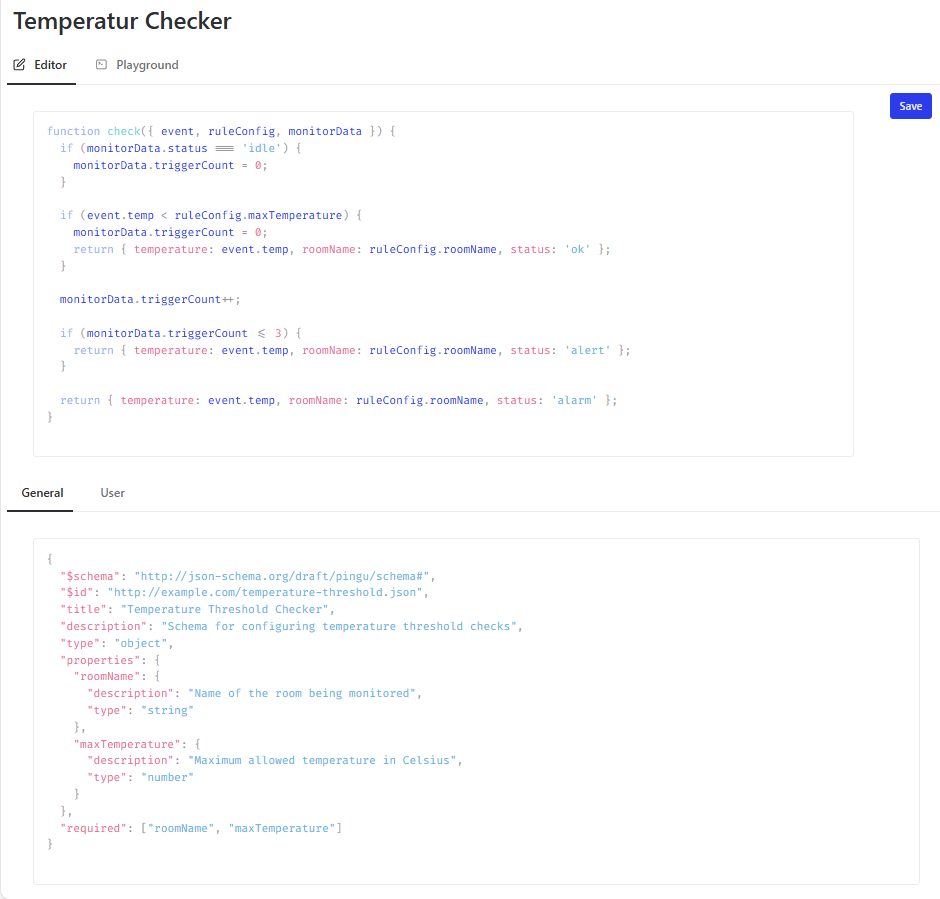
\includegraphics[width=1\linewidth]{function.png}
  \caption{Konfigurationskomponente einer Temperatur Checker Funktion}
  \label{fig:function}
\end{figure}


(Playground wird evtl. kurz beschrieben TBD)

Die Hauptkomponenten des Monitors wird noch beschrieben(TBD) mit einer Abbildung. 



\subsection{Problemstellung}

Info: Die Problemstellung wurde noch nicht angepasst auf das neue Kapitel 1.2 (TBD).

Basierend auf den Erkenntnissen und Einschränkungen des Vorprojekts IP5 sollen in dieser Bachelorarbeit die hardcodierten Komponenten reduziert werden. Ziel ist die Analyse und Umsetzung einer modularen Lösung, welche das Datenmodell als virtuelles Filesystem bereitstellt, um Anpassungen oder Erweiterungen am Datenmodell ohne Änderungen am Quellcode zu ermöglichen.Die entwickelte Lösung soll mit verschiedenen Datenstrukturen kompatibel sein und insbesondere die Abbildung komplexer IoT-Strukturen unterstützen. Dabei wird das spezifische Monidas-Datenmodell zunächst durch ein allgemeineres Modell ausgetauscht. Zur Validierung und Überprüfung der angestrebten Generalisierbarkeit wird am Ende der Arbeit das ursprüngliche Monidas-Datenmodell exemplarisch wieder integriert. Zusätzlich wird ein eigener Language Server implementiert, welcher erweiterte Funktionen wie Validierung, Autovervollständigung und Navigation im Editor bereitstellt und somit die Bearbeitung der Daten  unterstützt.

Ein erster Schritt zur Reduktion des Entwicklungsaufwandes wurde im Vorprojekt IP5 („Entwicklung einer VS-Code Extension zur Verwaltung von IoT-Daten in der Monidas-Plattform“) evaluiert. Im Rahmen eines Proof-of-Concept untersuchte das Projekt, ob eine alternative Benutzeroberfläche den bisherigen Prozess der Sensorkonfiguration vereinfachen und optimieren kann. Dazu wurde eine VS-Code Extension entwickelt, die Teile des bestehenden Monidas-Datenmodells in einer hierarchischen Baumstruktur (TreeView) darstellt. Diese Benutzeroberfläche ermöglicht die direkte Erstellung und Bearbeitung der IoT-Daten in der Entwicklungsumgebung mithilfe eines JSON-Editors. Obwohl der entwickelte Prototyp aus IP5 erste positive Ergebnisse lieferte, zeigte er zugleich zentrale Schwächen auf: Die implementierte Lösung basiert auf einer statischen Integration des Datenmodells („Hardcodierung“). Daher erfordert jede Anpassung oder Erweiterung des Datenmodells manuelle Eingriffe in den Quellcode. Diese Tatsache schränkt Erweiterbarkeit, Wartbarkeit und Skalierbarkeit der Lösung erheblich ein. Die starre und unflexible Implementierung erweist sich langfristig als ineffizient und fehleranfällig.

Aus den dargelegten Gründen ergibt sich die Notwendigkeit einer dynamischen, generischen und datenmodellgesteuerten Lösung. Diese Anforderungen bilden die Grundlage für den Monidas Code Assist Navigator.

\newpage
\subsection{Monidas Code Assist Navigator} 

Info: Hier versuche ich das entwickelte Resultat in einem Szenario zu beschreiben. Dieser Abschnitt muss noch angepasst werden auf die vorherigen Kapitel. (TBD)

\paragraph{Szenario}
Stellen Sie sich folgendes Szenario vor: 

Sie sind Teil eines Entwicklerteams, das eine IoT-basierte Anwendung entwickelt. Aufgrund begrenzter zeitlicher und personeller Ressourcen ist es Ihrem Team jedoch nicht möglich, eine Benutzeroberfläche für die Konfiguration der Sensoren zu implementieren.

Um dennoch die ersten Sensoren zu verwalten, benötigen Sie eine Lösung, die ohne zusätzlichen Entwicklungsaufwand einsatzbereit ist. Genau hier setzt der im Rahmen dieser Arbeit entwickelte Monidas Code Assist Navigator an.

Zu Beginn definieren Sie innerhalb des Navigators das Schema Ihrer Anwendungsdomäne. Sobald das Datenmodell definiert und die Datenbank eingerichtet wurde, ist der Monidas Code Assist Navigator einsatzbereit.


%Um die Daetn zu verwalten muss eine Kompontente des Navigarotr insstaliert werden. ieren Sie zunächst eine dafür entwickelte VS-Code-Extension (Name noch festzulegen). Nach Sie alle definierten Sensoren über ein virtuelles Dateisystem verwalten. Das zugrunde liegende Datenmodell wird hierbei als hierarchischer Baum mit Ordnern und Dateien dargestellt. Wenn Sie eine dieser Dateien öffnen, erscheint automatisch der zugehörige Editor.

%An diesem Punkt unterstützt Sie die zweite Extension (Name noch festzulegen), welche als Editorunterstützung fungiert. Diese Extension erleichtert die Navigation innerhalb des virtuellen Dateisystems und bietet hilfreiche Funktionen wie automatisches Vervollständigen, Validieren von Eingaben und Anzeigen erforderlicher Attribute an. Dadurch wird die Verwaltung der IoT-Daten zusätzlich vereinfacht.


\subsection{Forschungsfragen}

Welche Architekturentscheidungen sind erforderlich, um den „Code Assist Navigator“ umzusetzen?

Welche Auswirkungen hat die Umsetzung des „Code Assist Navigators“ auf die Skalierbarkeit, Erweiterbarkeit und Flexibilität der bestehenden Monidas-Plattform, insbesondere im Hinblick auf das zugrundeliegende Datenmodell?

Wo liegen die technischen sowie konzeptionellen Grenzen des „Code Assist Navigators“ bei der Verarbeitung, Darstellung und Navigation komplexer und tiefer Datenmodelle?

\newpage
\subsection{Abgrenzung}
%Im Rahmen dieser Arbeit werden folgende Themenbereiche nicht behandelt. Die entwickelte Lösung wird nicht in das Produktivsystem von Monidas integriert. Es findet keine Anbindung an die bestehende Webplattform oder das Backend statt. Die Evaluation erfolgt ausschliesslich anhand des Datenmodells, ohne produktive Abläufe zu beeinflussen.

% Nicht berücksichtigt werden ausserdem Funktionen zur gleichzeitigen Nutzung durch mehrere Benutzer, die Benutzerverwaltung, Authentifizierungsprozesse sowie die Rechtevergabe. Auch Themen wie Datensicherheit, Performanceoptimierung, Datenmigration oder die Anbindung externer Systeme sind nicht Bestandteil dieser Arbeit.

Im Rahmen dieser Arbeit werden einige Themenbereiche bewusst ausgeklammert. Die entwickelte Lösung wird nicht in das Produktivsystem von Monidas integriert, und es erfolgt keine Anbindung an die bestehende Platform. Die Evaluation der Lösung basiert ausschliesslich auf dem Datenmodell.

Ebenfalls nicht berücksichtigt werden Funktionen zur Mehrbenutzernutzung, zur Benutzerverwaltung sowie zu Authentifizierungs- und Autorisierungsprozessen. Themen wie Datensicherheit, Performanceoptimierung oder Datenmigration liegen ebenfalls ausserhalb des Umfangs dieser Bachelorarbeit.

\subsection{Leserführung}

%Diese Bachelorarbeit ist in fünf Kapitel gegliedert. Kapitel 1 beschreibt die Ausgangslage und Problemstellung sowie einen Überblick zur entwickelten Lösung. Um den Lesenden einen verständlichen Einstieg in die Architektur zu ermöglichen, zeigt \textbf{Abbildung 1.1} eine vereinfachte Übersicht der entwickelten VS Code Extension. Diese Architektur besteht aus zwei zentralen Komponenten: der \textbf{Editorunterstützung (LSP-Komponenten)} und dem \textbf{Datenzugriff und der Verwaltung (VFS-Komponenten)}. Beide Komponenten kommunizieren über das Backend mit der Datenbank.


Info: Die Leseführung wird durch diese Darstellung unterstützt. Feedback wäre hilfreich, ob die aktuelle Darstellung zu detailliert ist und weiter reduziert werden sollte. 

\begin{figure}[H]
  \centering
  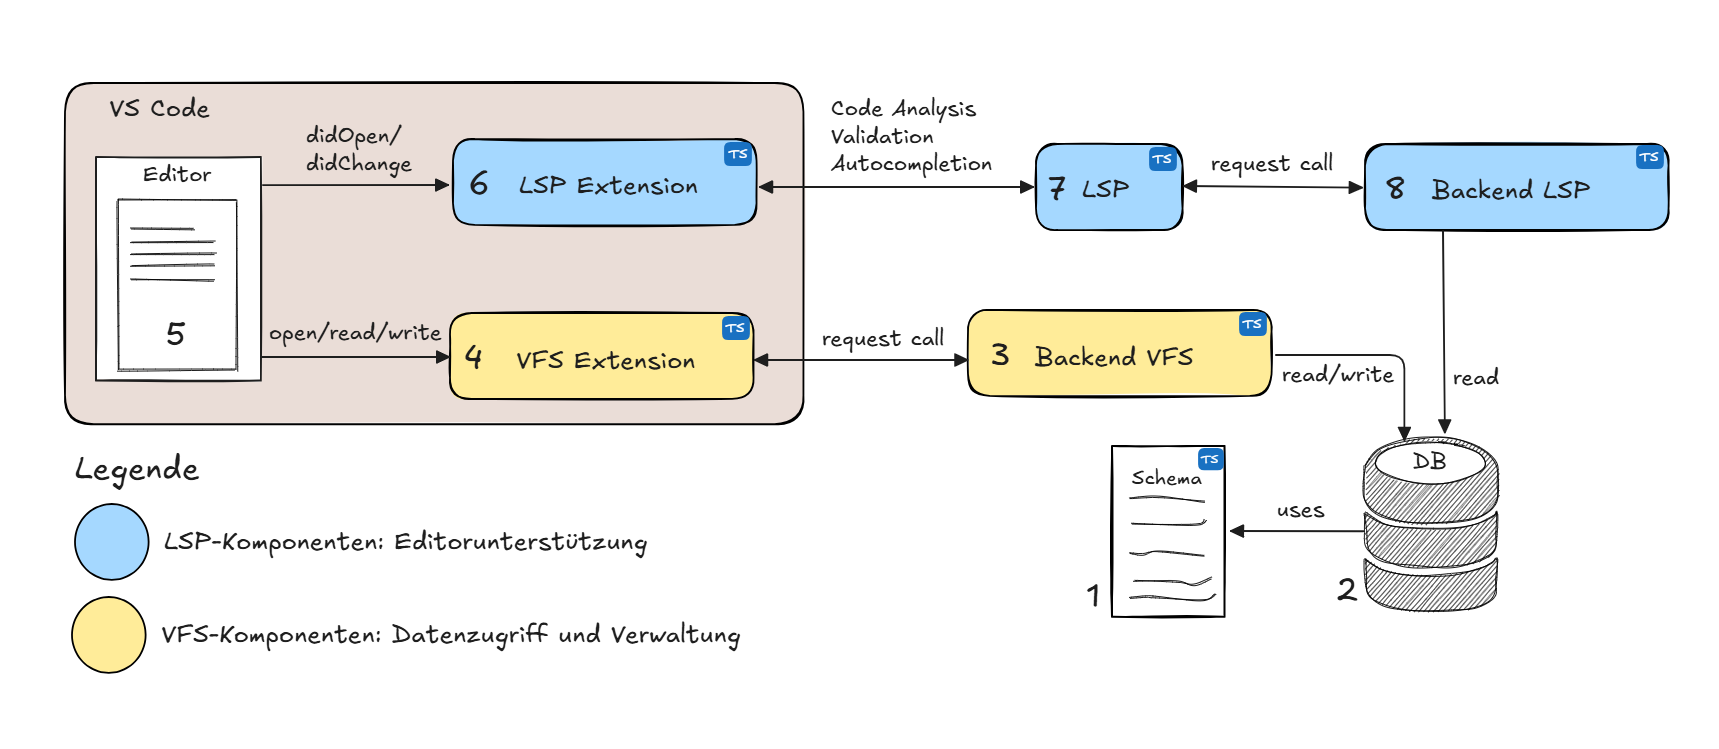
\includegraphics[width=\linewidth]{arch_simple.png}
  \caption{Architekturübersicht der implementierten Lösung}
  \label{fig:arch_simple}
\end{figure}


%Kapitel 2 widmet sich der Monidas-Plattform. Dort wird veranschaulicht, wie die Plattform aufgebaut ist und welche Technologien dabei verwendet werden. Zur besseren Verständlichkeit wird ein vereinfachtes Domänenmodell eingeführt und gezeigt, wie dieses in Form eines Schemas definiert wird. Dieses Schema bildet gleichzeitig die technische Grundlage der in der entwickelten VS Code Extension (Monidas Code Assist Navigator) verwendeten Technologien.

%Im Kapitel 3 steht das Schema der Datenbank im Mittelpunkt. Hier wird erläutert, weshalb das Schema für die Einführung des virtuellen Filesystems angepasst werden musste. Zusätzlich werden die selbst implementierten Constraints vorgestellt und deren Nutzen bei der Sicherstellung der Datenintegrität erläutert. Ein vereinfachtes Datenmodell aus dem Bereich E-Commerce dient als Referenzbeispiel für alle nachfolgenden Kapitel. Die Integration des ursprünglichen Monidas-Datenmodells erfolgt exemplarisch am Ende der Arbeit, um die Generalisierbarkeit der Lösung zu überprüfen. Abschliessend werden verschiedene Lösungsansätze präsentiert, wie das Schema zur Laufzeit analysiert und für die Komponenten VFS und LSP aufbereitet wird.

%Kapitel 4 beschäftigt sich mit dem virtuellen Filesystem. Im Vordergrund stehen dabei die VFS-Komponenten (4 und 3), welche eine dynamische Darstellung und Verwaltung der komplexen IoT-Daten ermöglichen.

%Kapitel 5 erläutert die Editorunterstützung durch die LSP-Komponenten (6, 7 und 8). Hier werden erweiterte Funktionen wie Validierung, Autovervollständigung und Navigation vorgestellt, welche eine effiziente und benutzerfreundliche Bearbeitung der IoT-Daten im Editor gewährleisten.

%Diese Struktur der Arbeit stellt sicher, dass die Lesenden eine klare Orientierung über die wesentlichen Inhalte erhalten und den Aufbau der entwickelten Lösung nachvollziehen können.
